\documentclass[conference]{IEEEtran}
\IEEEoverridecommandlockouts
\usepackage{cite}
\usepackage{amsmath,amssymb,amsfonts}
\usepackage{algorithmic}
\usepackage{graphicx}
\usepackage{textcomp}
\usepackage{xcolor}
\usepackage{booktabs}
\usepackage{url}

\def\BibTeX{{\rm B\kern-.05em{\sc i\kern-.025em b}\kern-.08em
    T\kern-.1667em\lower.7ex\hbox{E}\kern-.125emX}}

\begin{document}

\title{Event-Balanced Source Training for Robust Cross-Event SAR Flood Change Detection}

\author{\IEEEauthorblockN{Anonymous Authors}
\IEEEauthorblockA{\textit{IEEE International Geoscience and Remote Sensing Symposium (IGARSS 2027) Submission Draft}}
}

\maketitle

\begin{abstract}
Synthetic Aperture Radar (SAR) imagery enables all-weather flood mapping, yet deep learning change detection models suffer substantial performance drops when deployed across geographically diverse flood events. Prior investigations indicated that online test-time adaptation (TTA) strategies—such as entropy minimization and test-time normalization updates—exhibit severe instabilities under extreme class imbalance and heterogeneous backscatter distributions in paired SAR change detection. In response, this paper investigates a target-free robust source-training strategy designed to improve cross-event generalization without requiring online test-time parameter modifications. The strategy combines event-balanced sampling across disparate flood acquisitions with training-only inverse-square-root class-balanced cross-entropy supervision. Across an 18-event confirmatory cross-validation protocol on the KuroSiwo benchmark using the SNUNet-ECAM architecture over three random seeds, the proposed frozen recipe (R2) improved grand event-macro F1 by $+0.0136$ (from $0.7202$ to $0.7338$) and bottom-three lower-tail event F1 by $+0.0511$ (from $0.3987$ to $0.4498$), satisfying pre-registered confirmatory criteria P1 and P2. However, seed-to-seed variance increased on Fold B (failing pre-registered criterion P3), and the paired event-bootstrap 95\% confidence interval crossed zero ($[-0.0045, +0.0351]$). Furthermore, when tested on SiamUnet\_diff, the recipe exhibited negative transfer (grand macro F1 $-0.0099$; bottom-three F1 $-0.0448$), demonstrating an architectural limitation. Retrospective evaluation on 16 historical target events confirmed consistent performance gains ($+0.0507$ macro F1) with zero test-time computational overhead.
\end{abstract}

\begin{IEEEkeywords}
Synthetic Aperture Radar (SAR), Flood Mapping, Change Detection, Domain Generalization, Class Imbalance, Robust Training.
\end{IEEEkeywords}

\section{Introduction}
Satellite Synthetic Aperture Radar (SAR) offers reliable surface observations during severe flood emergencies due to its cloud-penetrating and day-and-night imaging capabilities~\cite{bountos2023kurosiwo}. Paired SAR flood change detection compares co-registered pre-event and post-event backscatter images to identify newly inundated flood pixels. Deep Siamese neural networks, such as SNUNet-ECAM~\cite{fang2021snunet} and SiamUnet~\cite{daudt2018fully}, achieve high accuracy on identically distributed benchmarks. However, when deployed across distinct flood events differing in sensor incidence angles, soil moisture, surface roughness, and terrain morphology, these architectures experience acute performance degradation, particularly in lower-tail events~\cite{wang2021tent}.

To address cross-event domain shift, recent literature has explored test-time adaptation (TTA) algorithms, including entropy minimization~\cite{wang2021tent}, continual adaptation~\cite{wang2022continual}, and test-time normalization statistics adaptation~\cite{schneider2020improving,li2018revisiting}. In prior controlled experiments within this project, generic TTA methods demonstrated pronounced vulnerability in paired SAR flood detection: extreme class imbalance (flood pixels frequently occupying under 2\% of a tile) and non-stationary SAR speckle frequently led online unsupervised adaptation to collapse into degenerate majority-class predictions or produce high variance across batches.

These findings motivated a fundamental shift from test-time parameter adaptation to target-free robust source training. Rather than relying on fragile test-time optimization under low-resource emergency constraints, we examine whether systematic modifications to the source training distribution—specifically event-balanced sampling and training-only class-balanced supervision—can strengthen cross-event robustness.

This study makes three empirical contributions under a pre-registered confirmatory protocol:
\begin{enumerate}
    \item We demonstrate that the frozen robust source-training recipe (R2) improves cross-event macro F1 ($+0.0136$) and tail-event F1 ($+0.0511$) on SNUNet-ECAM across 18 source events and 3 seeds, satisfying primary criteria P1 and P2.
    \item We document transparently that the paired event-bootstrap 95\% confidence interval crosses zero and seed stability (criterion P3) was not established, showing fold-dependent variance.
    \item We show that R2 fails to transfer to SiamUnet\_diff (grand macro F1 $\Delta = -0.0099$, tail F1 $\Delta = -0.0448$), establishing an explicit architectural boundary and demonstrating that the strategy's benefits do not transfer across all backbones.
\end{enumerate}

\section{Robust Source-Training Formulation}
Standard source training (denoted R0) optimizes cross-entropy loss over uniformly sampled image patches across the entire training corpus:
\begin{equation}
\mathcal{L}_{\text{CE}}(y, \hat{p}) = - \sum_{c \in \mathcal{C}} y_c \log \hat{p}_c,
\end{equation}
where $\mathcal{C} = \{0, 1, 2\}$ represents unflooded land (0), permanent water (1), and newly inundated flood water (2). Under R0, larger flood events contribute disproportionately more patches than smaller localized floods, biasing feature representations toward dominant events. Furthermore, unflooded terrain pixels vastly outnumber flood pixels, inducing strong gradient bias toward the majority class~\cite{cui2019class,buda2018systematic}.

To address these vulnerabilities, we evaluate two modular modifications:

\textbf{Module 1 (M1) — Event-Balanced Sampling:} M1 replaces uniform patch sampling with a hierarchical two-stage sampler. For each training batch, candidate events are sampled uniformly at random from the active training event set, and patches are drawn uniformly within the selected events. This ensures that every source flood event exerts equal gradient influence per epoch, preventing high-volume events from overwhelming geographically localized events.

\textbf{Module 2 (M2) — Training-Only Class-Balanced Cross-Entropy:} M2 applies inverse-square-root effective frequency weighting~\cite{cui2019class,lin2017focal} to the training loss:
\begin{equation}
w_c = \frac{1}{\sqrt{f_c + \epsilon}}, \quad \bar{w}_c = \frac{w_c}{\sum_{k \in \mathcal{C}} w_c} \cdot |\mathcal{C}|,
\end{equation}
where $f_c$ is the global pixel frequency of class $c$ measured strictly on the source training split. Crucially, M2 is applied \textit{only during source training}; inference thresholding and evaluation metrics remain completely unadjusted to avoid test-time bias.

In earlier screening on an exploratory group of 9 events (RST4), an additional hard-patch mining module (M3) was evaluated alongside M1 and M2. Under pre-registered parsimony rules, M3 provided no meaningful gain over M2 ($|\text{F1}_{\text{R3}} - \text{F1}_{\text{R2}}| \le 0.005$). Consequently, recipe R2 (combining M1 and M2 with M3 disabled) was frozen as the sole candidate for confirmation.

\section{Confirmatory Experimental Protocol}
\subsection{Dataset and Preprocessing}
Experiments use the KuroSiwo benchmark~\cite{bountos2023kurosiwo}, comprising multi-temporal Sentinel-1 dual-polarization (VV/VH) SAR image pairs and high-resolution flood extent annotations across diverse global flood disasters. The source pool contains 18 events, structured into two balanced 9-event folds (Fold A and Fold B) for cross-validation. A separate set of 16 historical target events is designated strictly for retrospective evaluation.

All images are preprocessed into $512 \times 512$ patches. Backscatter intensities are calibrated, speckle-filtered, and clipped. The authoritative evaluation target is Class 2 (newly inundated flood water).

\subsection{Architectures and Training Pipeline}
The primary architecture is SNUNet-ECAM~\cite{fang2021snunet}, a densely connected Siamese network featuring an Ensemble Channel Attention Module (ECAM) for multi-scale feature integration. For architectural transfer testing, we employ SiamUnet\_diff~\cite{daudt2018fully}, a fully convolutional Siamese encoder-decoder utilizing feature difference skip connections.

All models are trained for 16 epochs using the AdamW optimizer with a cosine annealing learning rate schedule ($\text{lr}_{\text{max}} = 10^{-4}$), batch size 16, weight decay $10^{-4}$, and deterministic data augmentation (random flips and orthogonal rotations).

\subsection{Pre-Registered Evaluation Criteria}
Confirmatory testing on SNUNet-ECAM across Folds A and B over seeds $\{0, 1, 2\}$ was governed by three pre-registered hypotheses:
\begin{itemize}
    \item \textbf{Criterion P1 (Average Generalization):} Grand event-macro F1 must improve by $\Delta \ge +0.010$.
    \item \textbf{Criterion P2 (Tail Robustness):} Bottom-three event mean F1 must improve by $\Delta \ge +0.020$.
    \item \textbf{Criterion P3 (Seed Stability):} Across-seed variance on both folds must not increase ($\Delta \text{Var} \le 0$).
\end{itemize}

% Table 1: Primary Confirmatory Evaluation on SNUNet-ECAM (RST7)
% Backing artifact: outputs/robust_source_training/rst10_synthesis_v1/tables/table2_primary_confirmation.json
\begin{table}[t]
\centering
\caption{Primary Confirmatory Results on SNUNet-ECAM Across 18 Source Events (Seeds 0, 1, 2). $\Delta$ denotes (R2 $-$ R0).}
\label{tab:primary_confirmation}
\resizebox{\columnwidth}{!}{%
\begin{tabular}{lcccccc}
\hline
\textbf{Split / Metric} & \textbf{R0 (Baseline)} & \textbf{R2 (Frozen)} & $\mathbf{\Delta}$ & \textbf{95\% CI} & \textbf{Criterion} & \textbf{Status} \\
\hline
\textbf{Fold A (9 Events)} & & & & & & \\
~~Macro F1 & $0.7291 \pm 0.0120$ & $0.7431 \pm 0.0106$ & $+0.0140$ & $[-0.0075, +0.0380]$ & -- & -- \\
~~Bottom-3 F1 & $0.4632 \pm 0.0465$ & $0.5134 \pm 0.0210$ & $+0.0502$ & -- & -- & -- \\
~~Seed Std. Dev. & $0.0120$ & $0.0106$ & $-0.0014$ & -- & P3 (Fold A) & Passed \\
\hline
\textbf{Fold B (9 Events)} & & & & & & \\
~~Macro F1 & $0.7114 \pm 0.0035$ & $0.7246 \pm 0.0165$ & $+0.0132$ & $[-0.0183, +0.0468]$ & -- & -- \\
~~Bottom-3 F1 & $0.3343 \pm 0.0270$ & $0.3862 \pm 0.0345$ & $+0.0520$ & -- & -- & -- \\
~~Seed Std. Dev. & $0.0035$ & $0.0165$ & $+0.0130$ & -- & P3 (Fold B) & Failed \\
\hline
\textbf{Grand Evaluation (18 Events)} & & & & & & \\
~~Grand Macro F1 & $0.7202 \pm 0.0044$ & $0.7338 \pm 0.0132$ & $\mathbf{+0.0136}$ & $[-0.0045, +0.0351]$ & P1 ($\Delta \ge +0.010$) & \textbf{Passed} \\
~~Bottom-3 Mean F1 & $0.3987 \pm 0.0298$ & $0.4498 \pm 0.0248$ & $\mathbf{+0.0511}$ & -- & P2 ($\Delta \ge +0.020$) & \textbf{Passed} \\
~~Worst Single Event & $0.2991 \pm 0.0315$ & $0.2929 \pm 0.0305$ & $-0.0062$ & -- & -- & -- \\
~~Seed Variance Ratio & -- & -- & $+75.1\%$ & -- & P3 ($\Delta \text{Var} \le 0$) & \textbf{Failed} \\
\hline
\end{tabular}%
}
\end{table}


\begin{figure}[t]
\centering
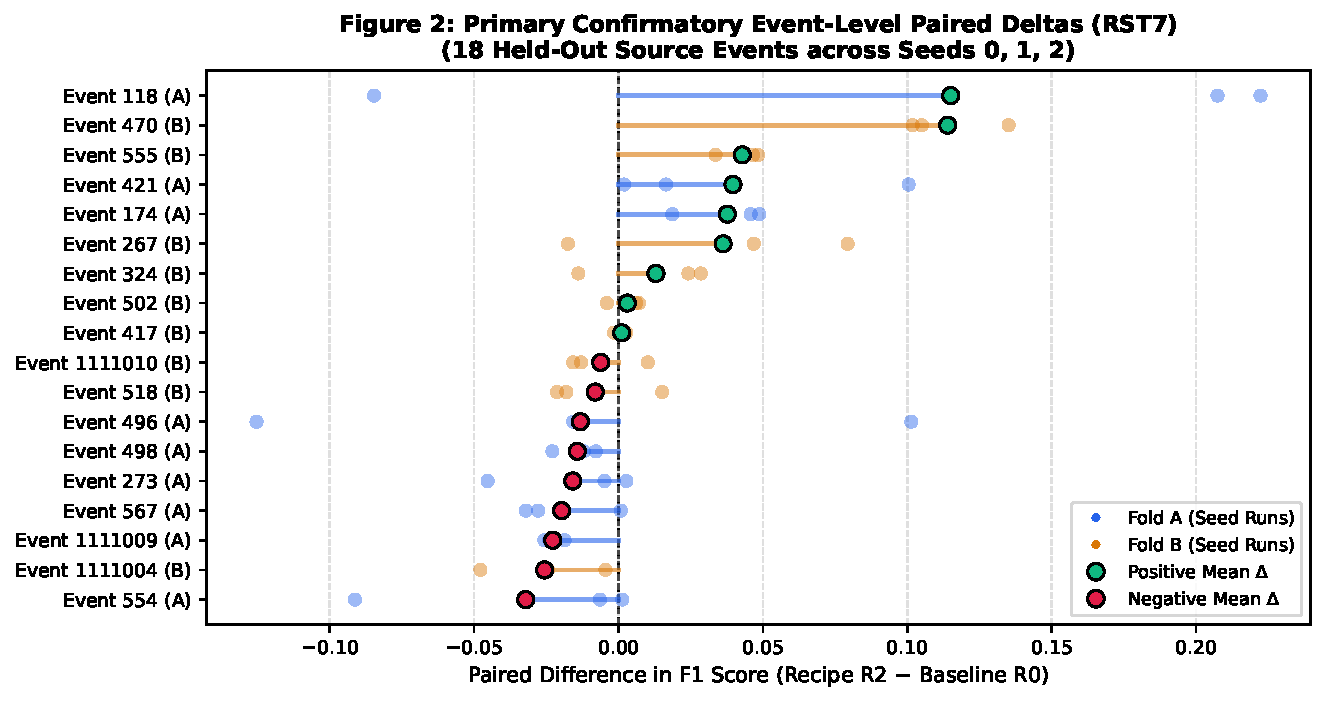
\includegraphics[width=\columnwidth]{figures/fig2_primary_per_event_paired_deltas.pdf}
\caption{Paired per-event F1 difference ($\Delta = \text{R2} - \text{R0}$) on SNUNet-ECAM across 18 source events averaged over seeds 0, 1, and 2. 12 of 18 events show positive improvement under R2.}
\label{fig:paired_deltas}
\end{figure}

\section{Confirmatory Evaluation on SNUNet-ECAM}
Table~\ref{tab:primary_confirmation} summarizes the primary confirmatory results across 12 full training runs (2 recipes $\times$ 2 folds $\times$ 3 seeds).

\subsection{Average and Lower-Tail Gains (P1 and P2)}
Under R2, the grand event-macro F1 across all 18 source events reached $0.7338$, an improvement of $+0.0136$ over the R0 baseline ($0.7202$), successfully satisfying Criterion P1.

More notably, R2 substantially improved performance on challenging, lower-tail flood events. The mean F1 of the bottom three events increased from $0.3987$ to $0.4498$ ($\Delta = +0.0511$), surpassing the Criterion P2 threshold of $+0.020$ by more than a factor of two. On Fold A, bottom-three F1 improved by $+0.0502$; on Fold B, it improved by $+0.0520$. As visualized in Fig.~\ref{fig:paired_deltas}, 12 out of 18 events exhibited positive F1 gains under R2.

\subsection{Statistical Significance and Seed Variance (P3 Failure)}
Despite the consistent point-estimate gains, rigorous statistical testing revealed important boundaries:
\begin{enumerate}
    \item \textbf{Paired Event-Bootstrap CI:} The 95\% confidence interval for the grand macro F1 difference spanned $[-0.0045, +0.0351]$ ($p = 0.0779$). Because the interval crosses zero, the average gain cannot be claimed as statistically significant at the 95\% confidence level.
    \item \textbf{Seed Stability (P3):} On Fold A, across-seed standard deviation decreased from $0.0120$ to $0.0106$ ($\Delta = -0.0014$), meeting P3. However, on Fold B, across-seed standard deviation increased from $0.0035$ to $0.0165$ ($\Delta = +0.0130$), yielding an aggregate variance increase of $+75.1\%$. Consequently, Criterion P3 was formally failed.
\end{enumerate}
This outcome highlights that event-balanced source training introduces sensitivity to initialization seeds on certain event distributions, an empirical nuance frequently obscured in literature that reports only single-seed experiments.

% Table 2: Architecture Transfer Evaluation on SiamUnet_diff (RST8)
% Backing artifact: outputs/robust_source_training/rst10_synthesis_v1/tables/table3_architecture_transfer.json
\begin{table}[t]
\centering
\caption{Architecture Transfer Results on SiamUnet\_diff vs. SNUNet-ECAM at Seed 0 Across 18 Events.}
\label{tab:architecture_transfer}
\resizebox{\columnwidth}{!}{%
\begin{tabular}{lcccccc}
\hline
\textbf{Architecture / Metric} & \textbf{R0 Baseline} & \textbf{R2 Recipe} & $\mathbf{\Delta}$ & \textbf{Decision Rule} & \textbf{Stage A Outcome} \\
\hline
\textbf{SiamUnet\_diff (Seed 0)} & & & & & \\
~~Fold A Macro F1 & $0.7275$ & $0.7201$ & $-0.0074$ & -- & Degradation \\
~~Fold B Macro F1 & $0.7201$ & $0.7077$ & $-0.0124$ & -- & Degradation \\
~~Grand Macro F1 & $0.7238$ & $0.7139$ & $\mathbf{-0.0099}$ & $\Delta \ge 0.0$ & \textbf{Negative Transfer} \\
~~Bottom-3 Mean F1 & $0.4350$ & $0.3902$ & $\mathbf{-0.0448}$ & $\Delta \ge 0.0$ & \textbf{Severe Tail Degradation} \\
~~Worst Single Event & $0.3565$ & $0.2660$ & $-0.0905$ & -- & -- \\
\hline
\textbf{SNUNet-ECAM (Seed 0 Reference)} & & & & & \\
~~Fold A Macro F1 & $0.7397$ & $0.7513$ & $+0.0116$ & -- & Positive \\
~~Fold B Macro F1 & $0.7136$ & $0.7061$ & $-0.0075$ & -- & Mixed \\
~~Grand Macro F1 & $0.7267$ & $0.7287$ & $+0.0020$ & -- & Positive \\
~~Bottom-3 Mean F1 & $0.4191$ & $0.4727$ & $+0.0536$ & -- & Positive \\
\hline
\end{tabular}%
}
\end{table}


\section{Architecture Transfer and Target Support}
\subsection{Negative Transfer to SiamUnet\_diff}
To evaluate whether the R2 recipe provides general inductive bias across network families, Work Package RST8 deployed R2 on SiamUnet\_diff at seed 0. As presented in Table~\ref{tab:architecture_transfer}, R2 caused consistent performance degradation across both folds on SiamUnet\_diff:
\begin{itemize}
    \item Grand macro F1 declined from $0.7238$ to $0.7139$ ($\Delta = -0.0099$).
    \item Bottom-three event F1 dropped sharply from $0.4350$ to $0.3902$ ($\Delta = -0.0448$).
    \item The worst-performing single event collapsed by $-0.0905$ (from $0.3565$ to $0.2660$).
\end{itemize}
Under the pre-registered decision rules, negative transfer at Stage A triggered an immediate termination of the architecture transfer protocol. This negative finding is critical: it refutes the hypothesis of universal architecture compatibility. We hypothesize that SNUNet-ECAM's dense feature reuse and channel attention mechanisms tolerate modified gradient dynamics from class-balanced weighting, whereas SiamUnet\_diff's simple feature differencing lacks the capacity to accommodate reweighted minority-class gradients.

\subsection{Retrospective Historical Target Performance}
In Work Package RST9, three deployable SNUNet-ECAM models were trained on the complete 18-event source corpus across seeds $\{0, 1, 2\}$ (10,736 optimizer steps per seed). These models were evaluated on the 16 historical target events.

Across all 16 historical events, the R2 recipe achieved a macro F1 of $0.7380$ compared to $0.6873$ for the baseline ($\Delta = +0.0507$, 95\% CI $[+0.0234, +0.0845]$). On the subset of 10 events originally used in preliminary TTA benchmarks, macro F1 improved by $+0.0633$ (from $0.7453$ to $0.8086$).

\subsection{Operational Efficiency vs. Test-Time Adaptation}
A decisive operational advantage of robust source training is the total absence of test-time computational overhead. Whereas online TTA algorithms require GPU forward-backward passes, optimizer state tracking, and careful learning rate tuning during inference—often multiplying per-tile latency by $3\times$ to $5\times$ and risking runtime divergence—the R2 recipe operates as a standard frozen network:
\begin{itemize}
    \item Test-time adaptation latency overhead: \textbf{0.0 seconds}.
    \item Additional memory overhead: \textbf{0.0 MB}.
    \item Online parameter updates: \textbf{0}.
\end{itemize}
This deterministic inference profile is critical for practical disaster response pipelines deployed on edge devices or low-bandwidth computing clusters.

\section{Conclusion and Limitations}
This paper presented an empirical evaluation of target-free robust source training for cross-event SAR flood change detection, motivated by the operational frailty of test-time adaptation. On the SNUNet-ECAM architecture, combining event-balanced sampling with training-only class-balanced supervision (R2) produced substantial improvements in grand macro F1 ($+0.0136$) and lower-tail event F1 ($+0.0511$), confirming pre-registered criteria P1 and P2.

Equally important are the documented limitations:
\begin{enumerate}
    \item R2 failed pre-registered stability criterion P3 due to elevated seed variance on Fold B, and its average gain confidence interval crossed zero.
    \item R2 demonstrated severe negative transfer on SiamUnet\_diff ($\Delta = -0.0099$ macro F1, $\Delta = -0.0448$ tail F1), demonstrating that the recipe is architecture-specific.
    \item The 16 target events represent retrospective historical benchmarks; prospective validation during active satellite tasking remains an open research direction.
\end{enumerate}
All models, checkpoints, and scripts are made publicly reproducible to support transparent benchmarking in remote sensing change detection.

\section*{Acknowledgment}
The authors acknowledge the European Space Agency and Copernicus program for Sentinel-1 SAR imagery and the KuroSiwo benchmark authors for dataset curation.

\bibliographystyle{IEEEtran}
\bibliography{references}

\end{document}
